\documentclass{beamer}

\usepackage[utf8]{inputenc}


%Information to be included in the title page:
\title{Movie Dataset Visualization}
%\author{Grigor Keropyan}
%\institute{Yerevan State University}
%\date{29/05/2020}

\author[Grigor] % (optional, for multiple authors)
{Grigor Keropyan\inst{1}}

\institute[YSU] % (optional)
{
	\inst{1}%
	Department of Mathematcis and Mechanics\\
	Yerevan State University
}

\date[2020] % (optional)
{29 may 2020}



\begin{document}

\frame{\titlepage}

\begin{frame}
\frametitle{About Dataset}

https://www.kaggle.com/rounakbanik/the-movies-dataset

\begin{figure}
	\centering
	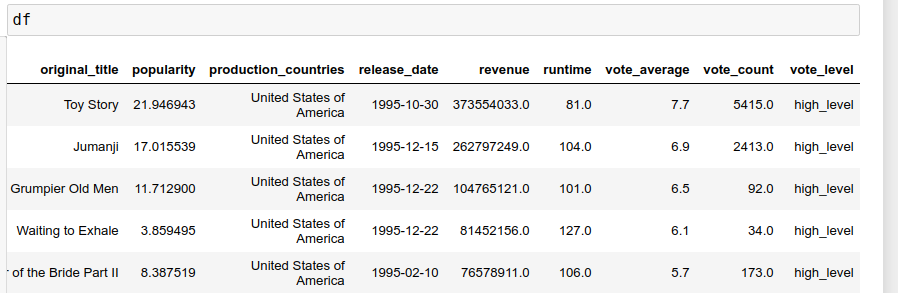
\includegraphics[width=0.7\linewidth]{dataset}
	\caption{Dataset}
	\label{fig:dataset}
\end{figure}

\end{frame}

\begin{frame}
\frametitle{Problem Definition}

Explore Movies dataset. Using data visualization techniques detect some dependencies between dataset features. Particularly, how popular is the movie depend on the what is the original language of it.

\end{frame}

\begin{frame}
\frametitle{Original language vs popularity}

Spanish? \newline
France? \\
English? \hfill \break
Armenian?


\end{frame}


\begin{frame}
\frametitle{Original language vs popularity}

\begin{figure}
	\centering
	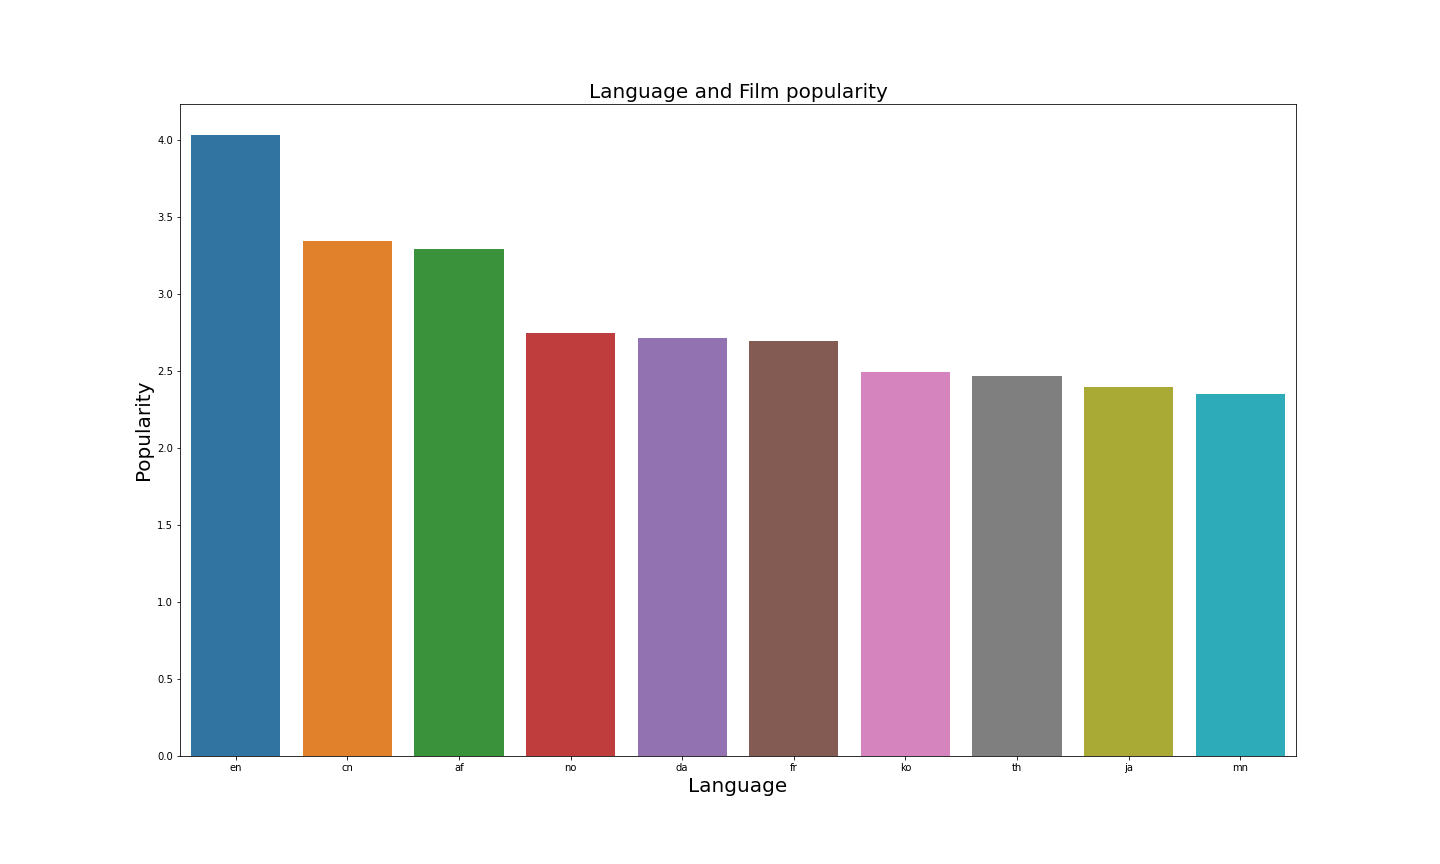
\includegraphics[width=1\linewidth]{language_film_pop}
	\caption{Movies popularity depends on their original language}
	\label{fig:pop_vs_language}
	
\end{figure}

\end{frame}

\begin{frame}
\frametitle{Genre count in movies}

\begin{figure}

	\centering
	\includegraphics[width=1.1\linewidth]{../plots/genre_count}
	\caption{Genre count in movies}
	\label{fig:genre_count}
	
\end{figure}

\end{frame}

\begin{frame}
\frametitle{Runtime vs Popularity}

\begin{figure}
	
	\centering
	\includegraphics[width=1.1\linewidth]{../plots/runtime_pop_line_graph}
	\caption{Runtime and Popularity connection}
	\label{fig:runtime_vs_pop}
	
\end{figure}

\end{frame}

\begin{frame}
\frametitle{Production countries}

\begin{figure}
	
	\centering
	\includegraphics[height=0.9\linewidth]{../plots/pie_prodaction_cointries_more_1000}
	\caption{Production countries more than 1000 movies. Pie plot}
	\label{fig:production_countries}
	
\end{figure}

\end{frame}


\begin{frame}
\frametitle{Genres in WordCloud}

\begin{figure}
	
	\centering
	\includegraphics[width=1.1\linewidth]{../plots/wordcloud_genre}
	\caption{wordcloud visualization of movie genres}
	\label{fig:genres}
	
\end{figure}

\end{frame}

\begin{frame}
\frametitle{Conclusion from the plots}

1. From the pie and bar plots we evidently understand that the most popular and movies come from the US. More than half of the movies are produced in United State Of America and most popular movies original language is in English. 
\end{frame}

\begin{frame}
\frametitle{Conclusion from the plots}

2. From the wordcloud and bar plots we evidently understand that the vast majority of movies
have a Drama genre.
\end{frame}

\begin{frame}
\frametitle{Conclusion from the plots}

3. Finally from the line graph we might be able to conclude that runtime of movies is connected with their popularity in some cases. 
\end{frame}

\begin{frame}
	\centering
	Thank you !
\end{frame}

\end{document}
